\section{Sjenčanje (shading)}

Sjenčanje je jedan od najbitnijih dijelova u 3D grafici. U ovome procesu određuje se boja i osvjetljenje pojedinoga fragmenta, te u konačnici i cijeloga modela. Iako ona ne mora nužno ovisiti o nekom izvoru svjetlosti, najčešće to nije slučaj.

Ovaj proces obrađuje se u fragment shader programu, te je u potpunoj kontroli korisnika. Ponekada, sjenčanje fragmenta se mora ponoviti više puta kako bi se postigao željeni slučaj. Takav način rada zove se iscrtavanje u više iteracija \footnote{engl. Multipass rendering}. Taj princip je korišten u postizanju toon shading efekta kako je objašnjeno dalje u ovome poglavlju.

Jedan od najjednostavnijih primjera sjenčanja je \emph{difuzno sjenčanje}, koji daje rezultat vrlo sličan onome kako ljudsko oko percipira predmete oko sobe. Jedan takav primjer prikazan je na slici \ref{fig:monkey-plastic}.


\begin{figure}[H]
\centering\fbox{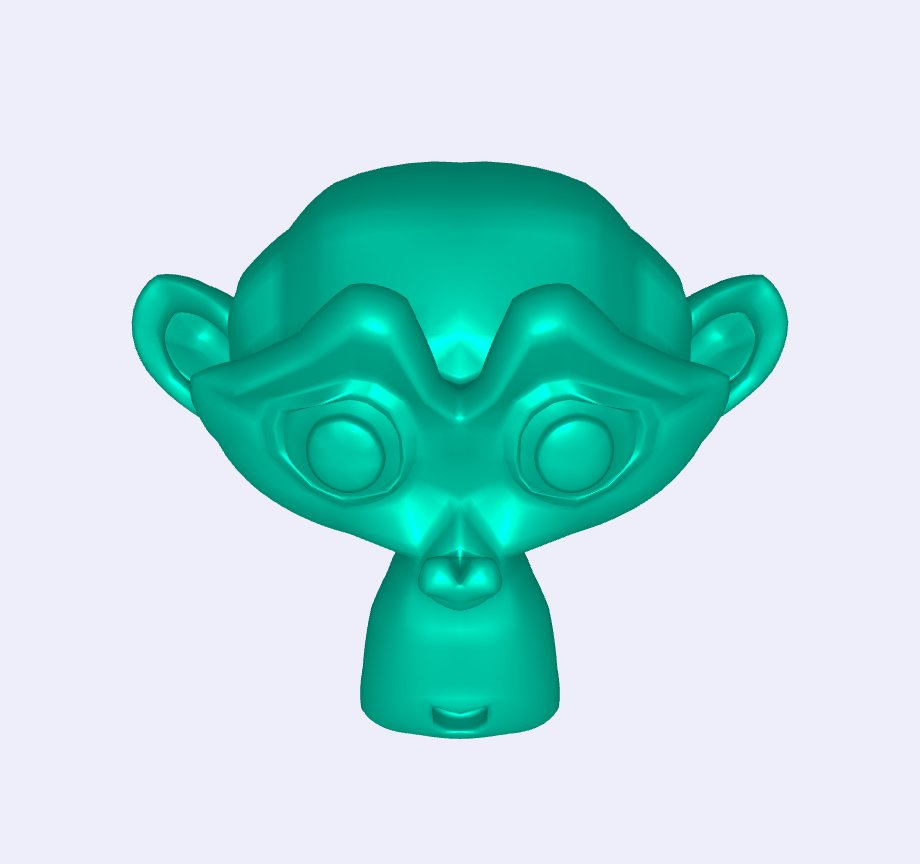
\includegraphics[scale=0.3]{monkey_plastic.png}}
\caption{Model osjenčan difuznom rasvjetom}
\label{fig:monkey-plastic}
\end{figure}

\emph{Difuzno sjenčanje} radi na sljedećem principu: intenzitet osnovna boja modela se pojačava, odnosno smanjuje u ovisnosti o kutu koju zatvara zraka svjetlosti i normale plohe na koju ta zraka pada. Kako je prikazano jednadžbom (\ref{eq:diffuse}), množenjem matrice normala plohe i matrice pozicije izvora svjetlosti, dobiva se faktor pojačanja. Za konačni rezultat, potrebno je faktor pojačanja pomnožiti sa osnovnom bojom modela.

\begin{equation}
\label{eq:diffuse}
C = (N \cdot L) * B
\end{equation}

Gdje je $N$ matrica normale plohe, $L$ matrica pozicije svijetla te $B$ matrica osnovne boje modela. 

\subsection{Toon-shading princip}

\emph{Toon-shading} naziv dolazi od engleske riječki \emph{cartoon}, što označava crtani film. Vrsta sjenčanja dobila je naziv zbog toga što se isti princip koristio u crtanim filmova kako bi je na jednostavan način prikaza 3D prostor.

Efekt se postiže na način da se modelu ocrtaju rubovi, te da se osjenča pojednostavljenim difuznim sjenčanjem - umjesto računanja faktora pojačanja za svaku pojedinu plohu, iste se dijele na zone čiji kut svijetla i normale pripada određenoj toleranciji. Na taj način na modelu se razlikuju samo tri do četiri tona osnovne boje modela. Primjer \emph{toon shading} načina sjenčanja prikazan je na slici \ref{fig:monkey-toonshaded}.

\begin{figure}[H]
\centering\fbox{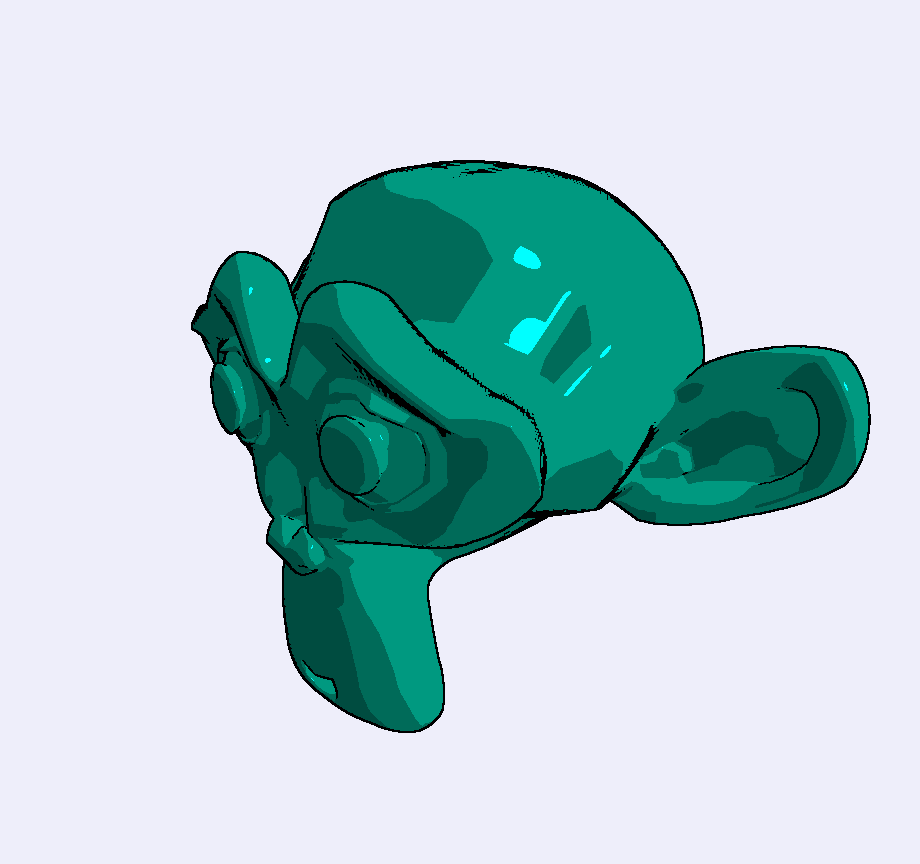
\includegraphics[scale=0.3]{monkey_toonshaded.png}}
\caption{Model sjenčan toon shaderom}
\label{fig:monkey-toonshaded}
\end{figure}

Kako bi bilo moguće postići efekt, potrebno je napraviti sljedeće koraka:

\begin{enumerate}
\item Ekstrakcija rubova
\item Pojednostavljeno difuzno sjenčanje
\item Stapanje slojeva u jednu sliku
\end{enumerate}

Budući da je \emph{fragment shader} zadužen za obradu samo jednoga \emph{fragmenta}, on nije svjestan svoje okoline. Točnije, prilikom obrade \emph{fragmenta} u \emph{fragment shaderu}, još nije određeno koji će biti njegovi susjedni \emph{fragmenti}. Kao posljedica toga dolazi činjenica da ekstrakciju rubova nije moguće odarditi u jednoj iteraciji. Iz tog razloga, \emph{toon shader} zahtjeva sjenčanje u više iteracija, točnije u njih četiri.

Kao posljedica toga dolaze performanse \emph{toon shadera}, koji je (u ovoj implementaciji) četiri puta sporiji od nekih jednostavnijih \emph{shadera}, poput difuznoga sjenčanje. Iako za današnje grafičke procesore ovo nije problem, uvijek je potrebno smanjiti kompleksnost gdje je to moguće. S tim ciljem, implementacija ovog algoritma biti će na način da se druga faza ekstracije rubova odvija u isto vrijeme kada i spajanje slojeva kako bi ukupan broj iteracija smanjili za jedan i ubrzali algoritam.

Sljedeća poglavlja opisuju svaki korak zasebno, te finalno spajanje slojeva u konačnu sliku koja se prikazuje korisniku.

\subsection{Iscrtavanje obrisa i rubova}

Prvi korak u \emph{toon shading}-u je ekstrakcija rubova. Iako postoji mnogo načina da se ovaj korak uradi, najjednostavniji je korištenjem \emph{Canny}-evog algoritma detekcije rubova. Budući da se ta metoda zasniva na pronalaženju razlike u kontrastu susjednih \emph{pixel}-a slike, potrebno je posebno prirediti sliku na kojoj će se detektor izvršiti.

Za te potrebe, u prvoj iteraciji iscrtana je slika modela u kojoj je boja svakoga \emph{pixel}-a predstavljena kao njegova udaljenost od kamere. U ovome slučaju, kamera je pozicionirana ispred samoga modela, tako da je udaljenost jednaka $z$ koordinati \emph{pixel}-a u koordinatnom sustavu. Rezultat ove iteracije prikazan je na slici \ref{fig:monkey-depth}.

\begin{figure}[H]
\centering\fbox{
\includegraphics[scale=0.3]{monkey_depth.png}}
\caption{Model s iscrtanom \emph{dubinom} pixel-a}
\label{fig:monkey-depth}
\end{figure}

Kako je prethodno napomenutu, samu detekciju rubova spojili smo u isto iteraciju sa samim spajanjem slojeva. No za potrebe analize, ovaj korak biti će objašnjen kao zasebna cjelina.

\emph{Canny}-ev algoritam detekcije rubova zasniva se na principu traženja razlike u kontrastu susjednih \emph{pixel}-a. U koliko ta razlika prelazi određenu vrijednost, smatra se da trenutni \emph{pixel} predstavlja rub na slici.

Kontrast između susjednih \emph{pixel}-a. određuje se tako da se susjedstvo piksela pomnoži sa \emph{maskom}. Zbroj svih elemenata dobivene matrice predstavlja vrijednost trenutno \emph{pixel}-a. Budući da \emph{Canny}-eva \emph{maska} radi samo u jednome pravcu, detekciju je potrebno izvršiti dva puta, za smjer posebno. \emph{Maske} korištene za ovu potrebu predstavljene su matricama $C_x$ i $C_y$ prikazanim u (\ref{eq:canny-kernel}).

\begin{equation}
\label{eq:canny-kernel}
	C_x = 
	\begin{bmatrix}
		1 & 0 & -1\\
		2 & 0 & -2\\
		1 & 0 & -1
	\end{bmatrix},
	C_y = 
	\begin{bmatrix}
		1 & 2 & 1\\
		0 & 0 & 0\\
		-1 & -2 & -1
	\end{bmatrix}
\end{equation}

U koliko sumu svih elemenata matrice $C_x$ predstavimo kao $s_x$, a sumu svih elemenaa matrice $C_y$ predstavimo kao $s_y$, tada se vrijednost trenutnoga \emph{pixel}-a $t$ računa prema \ref{eq:canny-threshold}.

\begin{equation}
\label{eq:canny-threshold}
	t = \sqrt{{s_x}^2 + {s_y}^2}
\end{equation}

Za svaki \emph{pixel} čija vrijednost $t$ prelazi zadanu granicu smatra se kao rub modela. Za potrebe algoritma, rubovi su iscrtani crnom bojom, dok su svi ostali \emph{pixel}-i ostavljeni bez boje, kako bi ih kasnije mogli lakše stopiti sa osjenčanom slikom.

Sama granična vrijednost nije unaprijed definira \emph{Canny}-evim algoritmom, već se proizvoljno određuje. Za potrebe ovog \emph{shader}-a, određeno je da će ta vrijednost iznositi $0.02$. Konačni rezultat prikazan je na slici \ref{fig:monkey-edges}.

\begin{figure}[H]
\centering\fbox{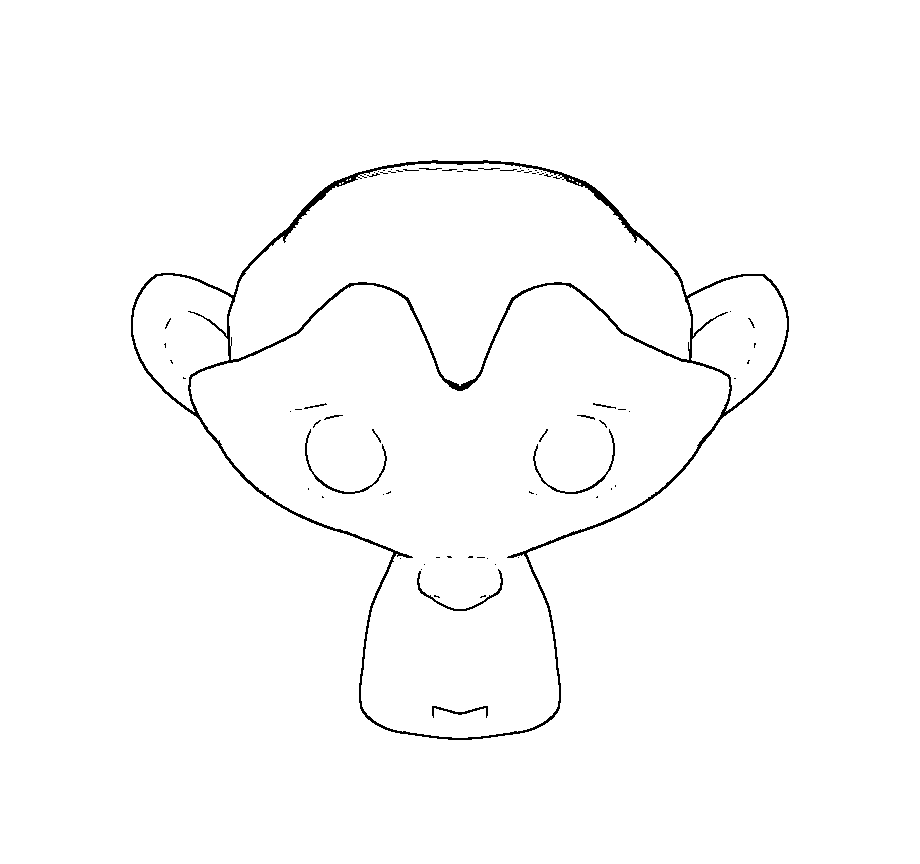
\includegraphics[scale=0.3]{monkey_edges.png}}
\caption{Model s iscrtanim obrisima}
\label{fig:monkey-edges}
\end{figure}

Kao što je vidljivo na slici \ref{fig:monkey-edges}, potrebno je napomenuti da ova metoda ne detektira sve rubove ispravno. No budući da u slučaju \emph{toon shader}-a rubovi služe samo za naglašavanje oblina, visoka preciznost nije potrebna, te je ovaj rezultat dovoljno dobar.

\subsection{Sjenčanje}

Za potrebe sjenčanja modela u \emph{toon shader}-u koristi se pojednostavljeno difuzno sjenčanje. Umjesto da se faktor pojačanja svjetlosti računa na osnovi svakoga fragmenta posebno, on je predodređen za dane intervale. Na taj način dobiva se model sa unaprijed predodređenim brojem tonova. Za potrebe ovog \emph{toon shader}-a određena su četiri tona osnovne boje.

Prvo je potrebno odrediti faktor pojačanja svjetlosti $t$ na isti način kao što se radi prilikom difuznog sjenčanja: Matricu $N$ koja predstavlja normale fragmenta potrebno je pomnožiti sa matricom $L$ koja predstavlja poziciju svjetla u prostoru kako je prikazano jednadžbom (\ref{eq:frgemnt-threshold}).

\begin{equation}
\label{eq:frgemnt-threshold}
t = N \cdot L
\end{equation}

No za razliku od (\ref{eq:diffuse}), gdje je faktor pomnožen izravno sa osnovnom bojom modela, ovdje ćemo konačni faktor pojačanja svjetlosti $t_f$ odrediti iz unaprijed određenih intervala na osnovu $t$ prema funkciji$f(t)$ opisanoj u (\ref{eq:toon-shading}).

\begin{equation}
\label{eq:toon-shading}
	f(t) =
	\begin{cases}
		0.5, & t \leq -0.6 \\
		0.7, & -0.6 < t \leq 0.1 \\
		1, & 0.1 < t \leq 0.97 \\
		3, & t > 0.97
	\end{cases}
\end{equation}

Konačni boju fragmenta $C$ dobivamo iz osnovne boje modela $B$ i konačnog faktora pojačanja svjetlosti $t_f$ prema (\ref{eq:toon-final-color}).

\begin{equation}
\label{eq:toon-final-color}
	C = t_f * B
\end{equation}

Primjenom navedenoga u korisničkom \emph{fragment shader}-u dobivamo rezultat prikazan na slici \ref{fig:monkey-toon}, koji predstavlja posljednji korak prije stapanja slojeva u jednu sliku.

\begin{figure}[H]
\centering\fbox{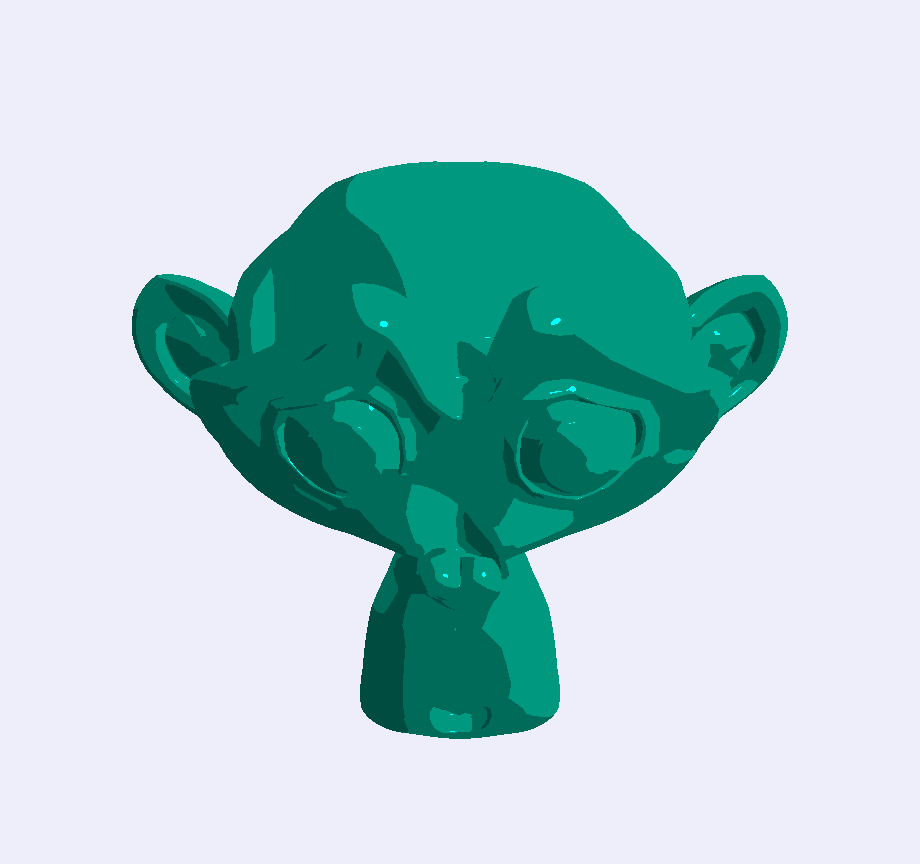
\includegraphics[scale=0.3]{monkey_toon.png}}
\caption{Osjenčani model}
\label{fig:monkey-toon}
\end{figure}

\subsection{Spajanje slojeva}

Rezultate prethodnih međukoraka potrebno je smjestiti u međuspremink, odnosno kao teksturu koja se prosljeđuje \emph{shader} programu u trećoj iteraciji. Te teksture prikazane su slikama \ref{fig:monkey-depth} i \ref{fig:monkey-toon}. Ovdje je potrebno raditi sa teksturama, jer jedino na taj način \emph{shader} programu možemo omogućiti rad nad susjedstvom \emph{pixel}-a.

Posljednja iteracija \emph{fragment shader}-a tada prvo provjerava dali se trenutni fragment treba tretirati kao rub. U koliko da, dodjeljuje mu se crna boja. U koliko ne, dodjeljuje mu se odgovarajuća boja sa prethodno osjenčanoga modela.

Na taj način postiže se efekt da je slika \ref{fig:monkey-edges} stavljena ispred \ref{fig:monkey-toon}, odnosno krajnji rezultat \emph{toon shading} algoritma.Taj rezultat prikazan je na slici \ref{fig:monkey-final}.

\begin{figure}[H]
\centering\fbox{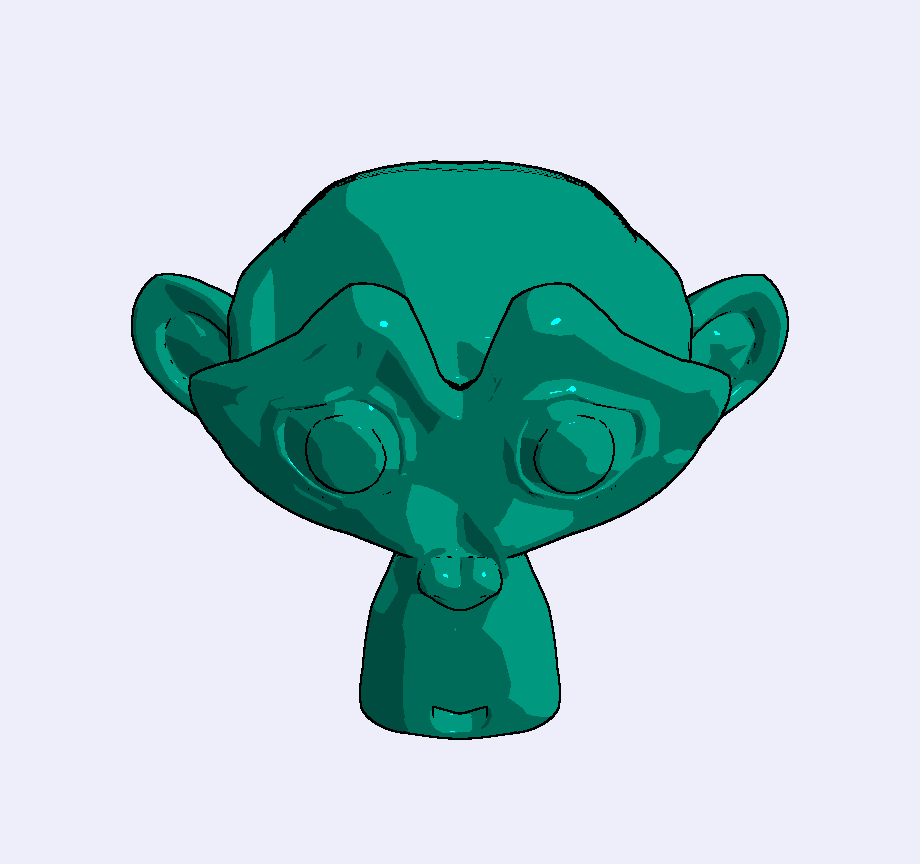
\includegraphics[scale=0.3]{monkey_final.png}}
\caption{Rezultat dobiven spajanjem slojeva}
\label{fig:monkey-final}
\end{figure}